\documentclass[12pt,titlepage]{article}

\usepackage[utf8]{inputenc}


% Set your default font encoding.
\usepackage[T1]{fontenc}

% Set default language priority order.
\usepackage[english]{babel}

% Set default margins.
\usepackage[a4paper,margin=25mm,headsep=5mm,headheight=12pt]{geometry}

\usepackage{amsmath,amssymb,amsfonts,amsthm}  % Mathematics
\usepackage{bbold}

\usepackage{hyperref} 
\hypersetup{colorlinks, 
    citecolor=black,
    filecolor=black, 
    linkcolor=black,
    urlcolor=black
      }

\usepackage{setspace}
\usepackage{graphicx}
\usepackage{subcaption}
\usepackage[separate-uncertainty=true]{siunitx} %Use this for writing SI units
\sisetup{
  range-phrase=--,
  detect-all,
  output-decimal-marker={.},
  range-units=single,
  per-mode=reciprocal,
  separate-uncertainty=false
}
\usepackage{physics} %A lot of useful short commands for writing math/physics
\usepackage{url}
\usepackage{verbatim}
\usepackage[toc,acronym]{glossaries}
\usepackage{booktabs} % For nice tables
\usepackage{fancyhdr} % For header and footer
\usepackage{lipsum}
\usepackage{lastpage} % For page counter
\usepackage{svg} % Makes it possible to use .svg files 
\usepackage{float} % Just [H] for placing figures
\usepackage{comment} % Use \begin{comment}
\usepackage{listings} % Enables source code listings
\usepackage{enumerate}
\usepackage{enumitem}
\definecolor{codegreen}{rgb}{0,0.75,0}
\definecolor{codegray}{rgb}{0.5,0.5,0.5}
\definecolor{codepurple}{rgb}{0.58,0,0.82}
\definecolor{backcolour}{rgb}{0.97,0.96,0.97}
\lstdefinestyle{mystyle}{
    backgroundcolor=\color{backcolour},   
    commentstyle=\color{codegreen},
    keywordstyle=\color{codepurple},
    numberstyle=\tiny\color{codegray},
    stringstyle=\color{magenta},
    basicstyle=\ttfamily\footnotesize,
    breakatwhitespace=false,         
    breaklines=true,                 
    captionpos=b,                    
    keepspaces=true,                 
    numbers=left,                    
    numbersep=5pt,                  
    showspaces=false,                
    showstringspaces=false,
    showtabs=false,                  
    tabsize=2
}

\lstset{style=mystyle}

% using inkscapefiles
\graphicspath{{figures/}}


%%%
\def\nameoflab{Beam up my quantum state, Scotty!}
\def\coursecode{FYST85}

\def\authorOne{Max Eriksson \& Lukas Nord}
\def\authorOneMail{maxerikss@gmail.com\\ Lukassigvard@gmail.com}
\def\headerName{M. Eriksson, L. Nord}

\def\supervisor{Peter Samuelsson}
\def\supervisorMail{peter.samuelsson@teorfys.lu.se}

\begin{document}
\begin{titlepage}
    \vspace*{\fill}	\newcommand{\HRule}{\rule{\linewidth}{0.5mm}}
	\center 
	\HRule\\[0.4cm]
	{\huge\bfseries \nameoflab}\\[0.4cm]
        {\Large\bfseries \coursecode}\\[0.1cm]
	\HRule\\[1.5cm]

    \large
    \textit{Author}\\
    \authorOne  \\ \texttt{\authorOneMail} \\

    \vspace{1cm}

    under the direction of \\ 
    \supervisor \\ \texttt{\supervisorMail}\\
    

    \vspace{1cm}
     
    Lund University\\
    Department of Physics
     
    
    \begin{figure}[H]
        \centering        
        
\includegraphics[width=6cm]{format/lund.png}
    \end{figure}
    
    \bigbreak
    \vfill
    \today
\end{titlepage}
%\pagestyle{empty}
%Header and footer
\pagestyle{fancy}
\fancyhead[L]{\footnotesize \textsc{\headerName}} %Change to your name
\fancyhead[R]{\footnotesize \textsc{\leftmark}}
\fancyfoot[R]{Page \thepage (\pageref{LastPage})}
\fancyfoot[C]{}


\tableofcontents
\clearpage
\vspace*{2cm}
\begin{figure}[H]
    \centering
    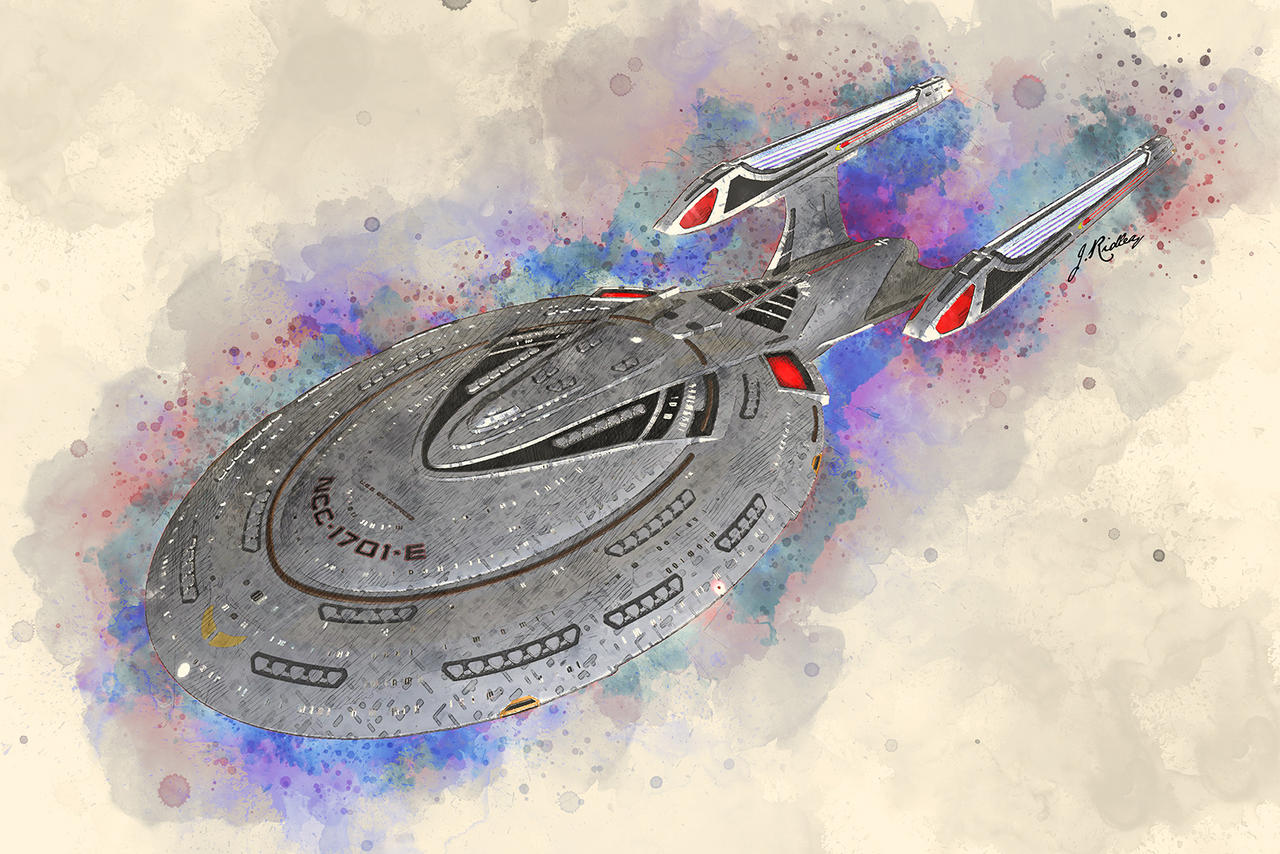
\includegraphics{figures/uss_enterprise.jpg}
    \vspace*{-8mm}
    \flushleft
    USS Enterprise \cite{uss}
\end{figure}
\vspace*{\fill}
\begin{center}
    \Large
    \textit{``I think I can safely say that nobody understands quantum mechanics.''} --- Richard P. Feynman
\end{center}
\vfill

\clearpage
\setcounter{page}{1}

\pagestyle{fancy}
\doublespacing

\section{Introduction}
\begin{mybox}{Bullet points}
    \begin{itemize}
        \item Quantum teleportation protocol
        \item Why is it needed?
        \item Areas of application, quantum communications, quantum computers
        \item what is needed to realize it on a large scale, i.e. quantum repeaters, memory...
        \item EPR-pairs and bell basis
    \end{itemize}
\end{mybox}
\subsection{Preliminaries}
In quantum teleportation the sender and receiver are referred to as Alice and Bob, and are denoted A and B respectively. Sometimes a third party is relevant which will be called Charlie and be denoted C.

\subsubsection{EPR-pairs and the Bell Basis}
An Einstein-Podolsky-Rosen-pair (EPR-pair) is a maximally entangled state of two qubits \cite{Nielsen:2010} which can be written as
\begin{equation}
    \ket{\Phi^\pm} = \frac{\ket{00} \pm \ket{11}}{\sqrt{2}} \quad \text{and} \ket{\Psi^\pm} = \frac{\ket{01} \pm \ket{10}}{\sqrt{2}}.\label{eq:epr}
\end{equation}
When measuring a quantum state the basis of measurement is important as this determines the possible outcome states. Common basis used are the computational basis, consisting of $\ket{0}$ and $\ket{1}$, and the Bell basis consisting of the EPR-pairs, also known as Bell states, seen in Eq. \eqref{eq:epr}. EPR-pairs and projective measurements in the Bell basis, henceforth called Bell measurements, play a crucial role in quantum teleportation protocols. \cite{Nielsen:2010}


\subsection{Quantum Teleportation Protocol}
Good source? \cite{Bennett:1993}

Let Alice have a particle with a normalized state $\ket{\phi} = \alpha \ket{0}_\phi + \beta \ket{1}_\phi$, which is unknown to her, that she wants to send to Bob. Sending the particle itself is rarely possible since Alice does not necessarily know where Bob located. She also cannot measure the particle to get accurate information since the particle is part of an unknown orthonormal set. To overcome these hurdles Alice can instead opt to send, or teleport, the state $\ket{\phi}$ to Bob. \cite{Bennett:1993}

To realize this teleportation both a classical channel and a non-classical channel will be used. The non-classical channel is made of an EPR-pair, where one particle is with Alice and one with Bob. Let Alice and Bob share the EPR-pair 
\begin{equation}
    \ket{\Psi^-}_{AB} = \frac{\ket{0}_A\ket{1}_B - \ket{1}_A\ket{0}_B}{\sqrt{2}}.
\end{equation}
The subscript denotes if Alice or Bob has the particle. Thus, the entire system is in the state 
\begin{align}
    \ket{\psi} &=\ket{\phi}\ket{\Psi^-}_{AB} \\ &= \frac{\alpha}{\sqrt{2}} (\ket{0}_\phi \ket{0}_A \ket{1}_B - \ket{0}_\phi \ket{1}_A \ket{0}_B) + \frac{b}{\sqrt{2}} (\ket{1}_\phi \ket{0}_A \ket{1}_B - \ket{1}_\phi \ket{1}_A \ket{0}_B)
\end{align}
Rewriting the products $\ket{x}_\phi\ket{x}_A$, that is the part of the system that is with Alice, using the Bell basis the system can be written as 
\begin{multline}
    \ket{\psi} = \frac{1}{2}\left[
        \ket{\Psi^-}_{\phi A} (-\alpha\ket{0}_B - \beta\ket{1}_B)   
        \ket{\Psi^+}_{\phi A} (-\alpha\ket{0}_B + \beta\ket{1}_B)\right.\\
        \left.\ket{\Phi^-}_{\phi A} (\alpha\ket{1}_B + \beta\ket{0}_B)
        \ket{\Phi^+}_{\phi A} (\alpha\ket{1}_B - \beta\ket{0}_B)
        \right]  
\end{multline}
That is, if Alice performs a Bell measurement the system will collapse into one of these terms. \cite{Bennett:1993}

Depending on the result of the measurement Bob will have the following states
\begin{align}
    A: \ket{\Psi^-}_{\phi A} &\longrightarrow B: -\alpha\ket{0}_B - \beta \ket{1}_B = -\ket{\phi}\\
    A: \ket{\Psi^+}_{\phi A} &\longrightarrow B: -\alpha\ket{0}_B + \beta \ket{1}_B = -Z\ket{\phi}\\
    A: \ket{\Phi^-}_{\phi A} &\longrightarrow B: \alpha\ket{1}_B + \beta \ket{0}_B = X\ket{\phi}\\
    A: \ket{\Phi^+}_{\phi A} &\longrightarrow B: \alpha\ket{1}_B - \beta \ket{0}_B = -iY\ket{\phi}\\
\end{align}
That is Bob will end up with a rotated version of $\ket{\phi}$. Thus, if Alice sends the result of her measurement classically to Bob he can perform the necessary rotation to obtain the state $\ket{\phi}$. The classical channel can be a generic broadcast, i.e. a radio, which essentially means that Alice doesn't need to know where Bob is exactly. 
\section{Teleportation of Complex Quantum Systems}
\begin{mybox}{Bullet points}
    \begin{itemize}
        \item What is a complex system?
        \item How does the protocol differ from simple systems?
        \item Why is it important to be able to teleport complex quantum systems?
        \item Theoretical and experimental limits
    \end{itemize}
\end{mybox}

\subsection{Complex Quantum Systems}
\section{Quantum Repeaters and Quantum Memory}
Quantum internet \cite{Azuma:2023}
\begin{mybox}{Bullet points}
    \begin{itemize}
        \item quantum repeater analogues to normal repeater?
        \item How to realize quantum memory 
        \item why do we need quantum memory for quantum repeaters
        \item how much does a quantum repeater reduce attenuation
        \item how good are today's quantum repeaters? 
    \end{itemize}
\end{mybox}

\subsection{Entanglement swapping}

Assuming that Alice and Bob are too far apart from each other to efficiently transport an entangled state between them,
an option is entanglement swapping. Assume that Alice and Bob each share an entangled state with the third part, Charlie.
These states would be $\ket{\phi}_{AC_1}$ and $\ket{\phi}_{BC_2}$. If Charlie now performs a simultaneus measurement on his two states, $C_1$ and $C_2$
Alice and Bobs qubits will end up in an entangled state. This is a way of propagating entaglement through a third part to achieve more reliable longer distance entaglement.

\subsection{Quantum memories (p.34)??}
\subsection{Quantum repeater protocol}
%No cloning but instead entanglement swapping
If long distance distribution of entanglement were to be achieved through optical fibers, one would experience an exponential loss of photons.
 To overcome this loss, quantum repeaters use heralded entanglement generation and entanglement swapping.
 Heralded entanglement generation involves establishing
 local Bell states between quantum memories and optical pulses at each party (e.g., Alice and a repeater node or two repeater nodes).
 The optical pulses are sent through fibers to a central station where a linear-optical Bell measurement is performed,
 projecting the pulses into an entangled Bell state with success probability 
 \begin{equation}
    p_g(l) = e^{-l/L_{\text{att}}}/2,
 \end{equation}
 where $l$ is the fiber length and $L_{\text{att}}$ is the attenuation length.
 Once neighboring parties share entanglement with a repeater node, entanglement swapping extends the entanglement between more distant parties.
 This is achieved via a Bell measurement on the quantum memories at the repeater node, succeeding with probability $p_s = 1/2$ in the ideal case.
 Without repeaters, directly linking Alice and Bob requires an average number of trials 
 \begin{equation}
    \langle T^{(0)}_{\text{tot}} \rangle = p_g(L)^{-1} = 2e^{L/L_{\text{att}}},
 \end{equation}
 which grows exponentially with the distance $L$. With a single repeater node located midway, entanglement generation is performed in parallel for Alice-to-repeater and repeater-to-Bob links,
 each requiring 
 \begin{equation}
    \langle T_g(L/2) \rangle = 2e^{L/(2L_{\text{att}})}
 \end{equation}
 trials on average. Successful swapping at the repeater node then connects Alice and Bob,
 requiring 
 \begin{equation}
    \langle T^{(1)}_{\text{tot}} \rangle \sim p_s^{-1} p_g(L/2)^{-1} = 2^2 e^{L/(2L_{\text{att}})}
 \end{equation}
 trials, providing a square-root improvement compared to the direct link.
 This process generalizes with $N_{\text{QR}} = 2^n - 1$ equally spaced repeater nodes, where each step reduces the entanglement distance to $L/(N_{\text{QR}} + 1)$,
 achieving a total trial count of
 \begin{equation}
    \langle T^{(N_{\text{QR}})}_{\text{tot}} \rangle \sim 2^{1+\log_2(N_{\text{QR}} + 1)} e^{L/((N_{\text{QR}} + 1)L_{\text{att}})},
 \end{equation}
 exponentially improving efficiency. While this idealized protocol assumes perfect operations and quantum memories, practical implementations must account for memory errors,
 imperfect operations, and accumulated errors, mitigated by advanced error-suppression techniques. Thus,
 quantum repeaters enable scalable quantum communication by mitigating photon loss and other imperfections over long distances.


\subsection{Experimental realizations???}
\section{Experimental Evidence}
Experimental evidence for quantum teleportation in quantum communications.
\begin{mybox}{Bullet points}
    \begin{itemize}
        \item Quantum teleportation has experimental evidence
        \item Experimental hurdles
    \end{itemize}
\end{mybox}
\subsection{Satellite Based}

1400 km \cite{Ren:2017}
\begin{mybox}{Bullet points}
    \begin{itemize}
        \item Protocol used
        \item distance
        \item technical difficulties and innovations
        \item what does this mean for quantum communications?
    \end{itemize}
\end{mybox}

The qubit system used in this experiment is based on the polarization of a photon with a state represented as $\ket{\chi}_1 = \alpha\ket{H}_1 + \beta\ket{V}_1$, with complex numbers
satisfying $\vert\alpha\vert² + \vert\beta\vert² = 1$ and $\ket{V}$ and $\ket{H}$ represents vertical and horizontal polarization respectively.
 At a ground station, two entangled photon pairs were prepared and one photon from each pair was
transmitted to a Satellite through a 130-mm diameter telescope with narrow beam divergence and high-precision tracking systmes to counteract the atmospheric turbulence.
The entangled pair of photons can be written as one of the Bell states,
\begin{equation}
    \ket{\psi^{+}}_{23} = (\ket{H}_2\ket{H}_3 + \ket{V}_2\ket{V}_3)/\sqrt{2},
\end{equation}
where photon 2 is the photon kept at the ground station and photon 3 was sent to the Satellite.

A joint measurement was one on the photon that was to be teleported and one of the entangled photons. This projects these photons into one of the Bell states.
The result from this measurment was then classically sent to the Satellite. This measurement forces the entangled pair into a new state. If this state is 
$\ket{\psi^{+}}_{12} = (\ket{H}_1\ket{H}_2 + \ket{V}_1\ket{V}_2)/\sqrt{2}$ the photon sent to the Satellite (photon 3) carries the state that photon 1 was in originally
and if the measured state is $\ket{\psi^{-}}_{12} = (\ket{H}_1\ket{H}_2 - \ket{V}_1\ket{V}_2)/\sqrt{2}$, the state of photon 3 is equivalent of the state of photon 1 shifted $\pi$.



\subsection{Fibre Network Based}
100 km \cite{Takesue:2015}. Metropolitan \cite{Valivarthi:2016}
\begin{mybox}{Bullet points}
    \begin{itemize}
        \item Protocol used
        \item distance
        \item technical difficulties and innovations
        \item what does this mean for quantum communications?
    \end{itemize}
\end{mybox} 

\section{Summary \& Conclusion}


\clearpage
\addcontentsline{toc}{section}{References}
\begin{singlespace}
\bibliographystyle{ieeetr}
\bibliography{references.bib}
\end{singlespace}

%\appendix 

\section{Appendix}

\end{document}